\documentclass{article}
\usepackage{graphicx} % Required for inserting images
\usepackage{url}
\usepackage{hyperref}
\usepackage{xcolor}
\usepackage{pdfpages}

\begin{document}

\begin{titlepage}
	\centering
    % --- Logo --- 
    
\includegraphics[width=\textwidth]{images/uliege-FSA.png} \\ [1 cm]

    % --- Header ---
	\textsc{\Large [INFO0085-1] - Compilers} \\ [0.4 cm]

    % --- Title ---
	\rule{\linewidth}{0.2 mm} \\[0.4 cm]
	{\Large \bfseries Compiler Project Report} \\
	\rule{\linewidth}{0.2 mm} \\[1.5 cm]

    % --- Teachers ---
	\begin{minipage}[t]{0.49\textwidth}
		\begin{flushleft} \large
		    \textbf{Teacher:} \\
                Pascal FONTAINE \\ [0.5 cm]
            \textbf{Teaching Assistant:} \\
                Roland GREFFE
		\end{flushleft}
	\end{minipage}
    \hfill 
	\begin{minipage}[t]{0.49\textwidth}
		\begin{flushright} \large
        \textbf{Authors:} \\
            Valérian WISLEZ (20200825)
		\end{flushright}
	\end{minipage}
    % --- Year ---
    \vfill
    \textsc{\Large Academic Year 2025-2026} \\ [1.0 cm]	
\end{titlepage}


\section{Introduction}

We will first give an overview of the project before moving into more details.

\paragraph{Name}

The compiler is named Khthon: derived from the greek $$\chi\theta o \nu \iota o \zeta$$ Pronounced "khthonios", it means "from the ground", metaphorically transforming high level language to a more ground-based IR. We thought it would be fun to make a parallel between the four steps of the compilation process and the four main places describing the underworld in greek mythology \footnote{\url{https://en.wikipedia.org/wiki/Greek\_underworld}}.

\paragraph{Repository}

You may consult the git repository \footnote{\url{https://github.com/valerian20024/khthon}} to find out more about the project than what has been posted on the submission platform. The content of the submission includes the source code, the report and a Doxygen documentation.

\paragraph{Participation}

The project has been done alone. Indeed, I have attended the course in 2024-2025, which allowed me to get some experience with the $3$ first steps. As I had had some troubles with team working last year

Unfortunately, I cannot state precisely how much time I have passed on the project, but I estimate it to be about $250$ hours, all in all. While that may seem a lot, it is mainly because I have used this project as an experimenting ground for learning C++. I was also quite passionate about it and willing to do it right. I have put some effort into readibility, architecture and correctness.

\paragraph{Statistics}

As of May 17, 2026, the project state can be summarized as follows: 

\begin{itemize}
    \item 29 source code files;
    \item roughly 7000 lines of code (4906 codes, 846 comments, 1314 blanks);
\end{itemize}

\section{Architecture}

We will now go over the architecture of the project and explain its main components.

\paragraph{Overview}

The project is using Flex, Bison and the LLVM C++ API. It follows a visitor pattern. Part of the lexer and the parser from last year have been reused, but we basically started fresh on this project.

The entrypoint of the program simply delegates to one of Driver's methods, which will perform the corresponding phase of compilation.

\paragraph{Lexical Analysis}
We use Flex's initial states to distinguish between three behaviors when scanning. 

\begin{itemize}
    \item Initial state: this corresponds to the base scanning mode, when reading VSOP code. The compiler will look for matching lexemes and execute the corresponding actions.
    \item Comments: when entering comments, the compiler should simply ignore everything until we reach the end of the comments. We are using a stack: pushing a new comment context when scanning the entry comments token and popping when scanning the end of comments token.
    \item Strings: the compiler should simply append to a string literal, and convert the necessary escaped characters to the expected format.
\end{itemize}

When the lexer has scanned a lexeme, generally it will call a function generated by Bison, in the form of \texttt{Parser::make\_TOKEN\_NAME}. This can effectively create a token in the parser and transfer the information.

The lexer will report errors when scanning wrong tokens and output descriptive messages. Thus we made some rules for error tokens and we catch them explicitly to return a precise error.

\paragraph{Syntax Analysis}

The grammar is mostly following what is described in the VSOP manual.
We have reused part of the grammar of the old project, so we did not encounter many shift/reduce or reduce/reduce conflicts. However, we have had some difficulties with Bison's error system since it would cause us some conflicts when trying to implement more error catching rules.

To be able to report errors using the same system as the rest of the program, we had to use macros calling \texttt{Driver}'s methods for logging errors. Then we usually create a dummy object to continue the parsing and catch more errors.

Finally we call in the \texttt{PrintVisitor} to sweep throught the AST and print each of the node to stdout.

\paragraph{Semantic Analysis}

We are using two symbol tables and visitors to populate them. The first symbol table is for classes, their fields and methods. The second is for variables and their scope. We were motivated by the fact that VSOP really seemed to have these two concepts that could live separately.

The first symbol tables uses the informations classes, which are designed to store and retrieve all the required information for further process, thereby forming the classes symbol table. For example, \texttt{ClassInfo} contains the class data and references to its \texttt{FieldInfo}s and \texttt{MethodInfo}s. 
We decided to use this approach because it seemed safer, as it really tries to be as general as possible, and to have the possibility to extend it in the future, for example with metadata.

The main classes are the following:
\begin{itemize}
    \item \texttt{SemanticChecker}: used as the main orchestrator: it performs the required semantic checks and logs errors. 
    \item \texttt{ClassManager}: has ownership of the class symbol tables and can perform operations on it.
    \item \texttt{ScopeManager}: has ownership of the variables symbol table and can perform operations on it.
    \item \texttt{ClassesVisitor}: visits the classes in the AST to populate the first symbol table.
    \item \texttt{TypesVisitor}: visits the whole AST and checks types conformance before updating the scope symbol table.
\end{itemize} 

Finally we call in the \texttt{PrintVisitor} to sweep throught the AST and print each of the node to stdout, adding a small annotation for types.

We were not able to completely finish this part. We prefered to move on to the code generation part first, but then we couldn't find the time to finish this one.

\paragraph{Code Generation}



\section{Capabilities}

Here is a review of what the code is capable of doing as well as its limitations.
\begin{itemize}
    \item Lexical Analysis: 39/39 tests passed. No further comment.
    \item Syntax Analysis: 50/55 tests passed. A few errors are not handled as we have had some troubles to understand and use Bison's error recovery system.
    \item Semantic Analysis: 67/79 and 126/151 tests passed.
    \item Code Generation: 6/38 tests passed. Khthon can produce an executable, link with the runtime and output some IR. It can print in the terminal, instanciate objects, call methods. However, further constructs are unfortunately not compiled. 
\end{itemize}


\section{Project improvements}
With more experience both in compiler design and in C++, there are many things to be improved, most notably:

\begin{itemize}
    \item Change the lexer to only take one keyword token and use a hash table to decide its content.
    \item Create a dedicated \texttt{ErrorLogger} class instead of putting the responsibility of error management to \texttt{Driver}. The errors could be more descriptive as well: using Bison's \texttt{location}, we could copy the line from the source file to indicate the user where it happened and clearly highlight the error.
    \item Creating more namespaces. As the code grew, \texttt{khthon::Type} is conflicting with \texttt{llvm::Type}. It would be a good time to start thinking out to split the code into meaningful namespaces.
    \item Push further the debugging mechanics when compiling to have accurate and clean logging of what's happening. For now it's a bit mingled and not standardized.
    \item More consistent use of C++ features, such as move semantics, or the order private and public members (more idiomatic in C++).
    \item \texttt{Driver::print\_diagnostics} should print them in order (line, column) when compiling in release mode and keep the original order when compiling in Debug mode. This was originaly planned but we didn't have time to make it.
    \item Work on the test script and pipeline its execution using e.g. Github actions (see the git repository).
    \item Methods could be reordered in a more logical way in some classes.
    \item In the lexer, I initially planned to check for numbers to be in range for 32 bits, but didn't have the time to do it.
    \item In the parser, add more 'dummy' factory methods to create actual dummies instead of relying on C++'s default initialization.
    \item And many more things ...
\end{itemize}

This project will outlive the scope of this course and I shall improve Khthon in my free time.

\section{Course improvements}
We now describe some features we think could improve the project in the future.

\paragraph{VSOP} we think adding a bit more VSOP examples in the PDF statements could help visualize the language, a bit like the linked list example. For example, there is no piece of code with a while loop. We think a bit more examples could help before actually reviewing the tests on the submission platform.

\paragraph{Updates}
We think updating the reference container by adding gdb to debug inside the container and using a more recent version of LLVM and clang could help students to get acquainted with recent versions of LLVM. It would make it easier to install LLVM on other machines instead of relying on the container.

\section{Use of AI Tools}
Mainly to help understand LLVM IR, discuss and refine code organization, help with some C++ concepts.

However, the code is mine.

\appendix

\section{Classes}

A document describing the classes hierarchy and where to find their interface and implementation is given afterwards. 

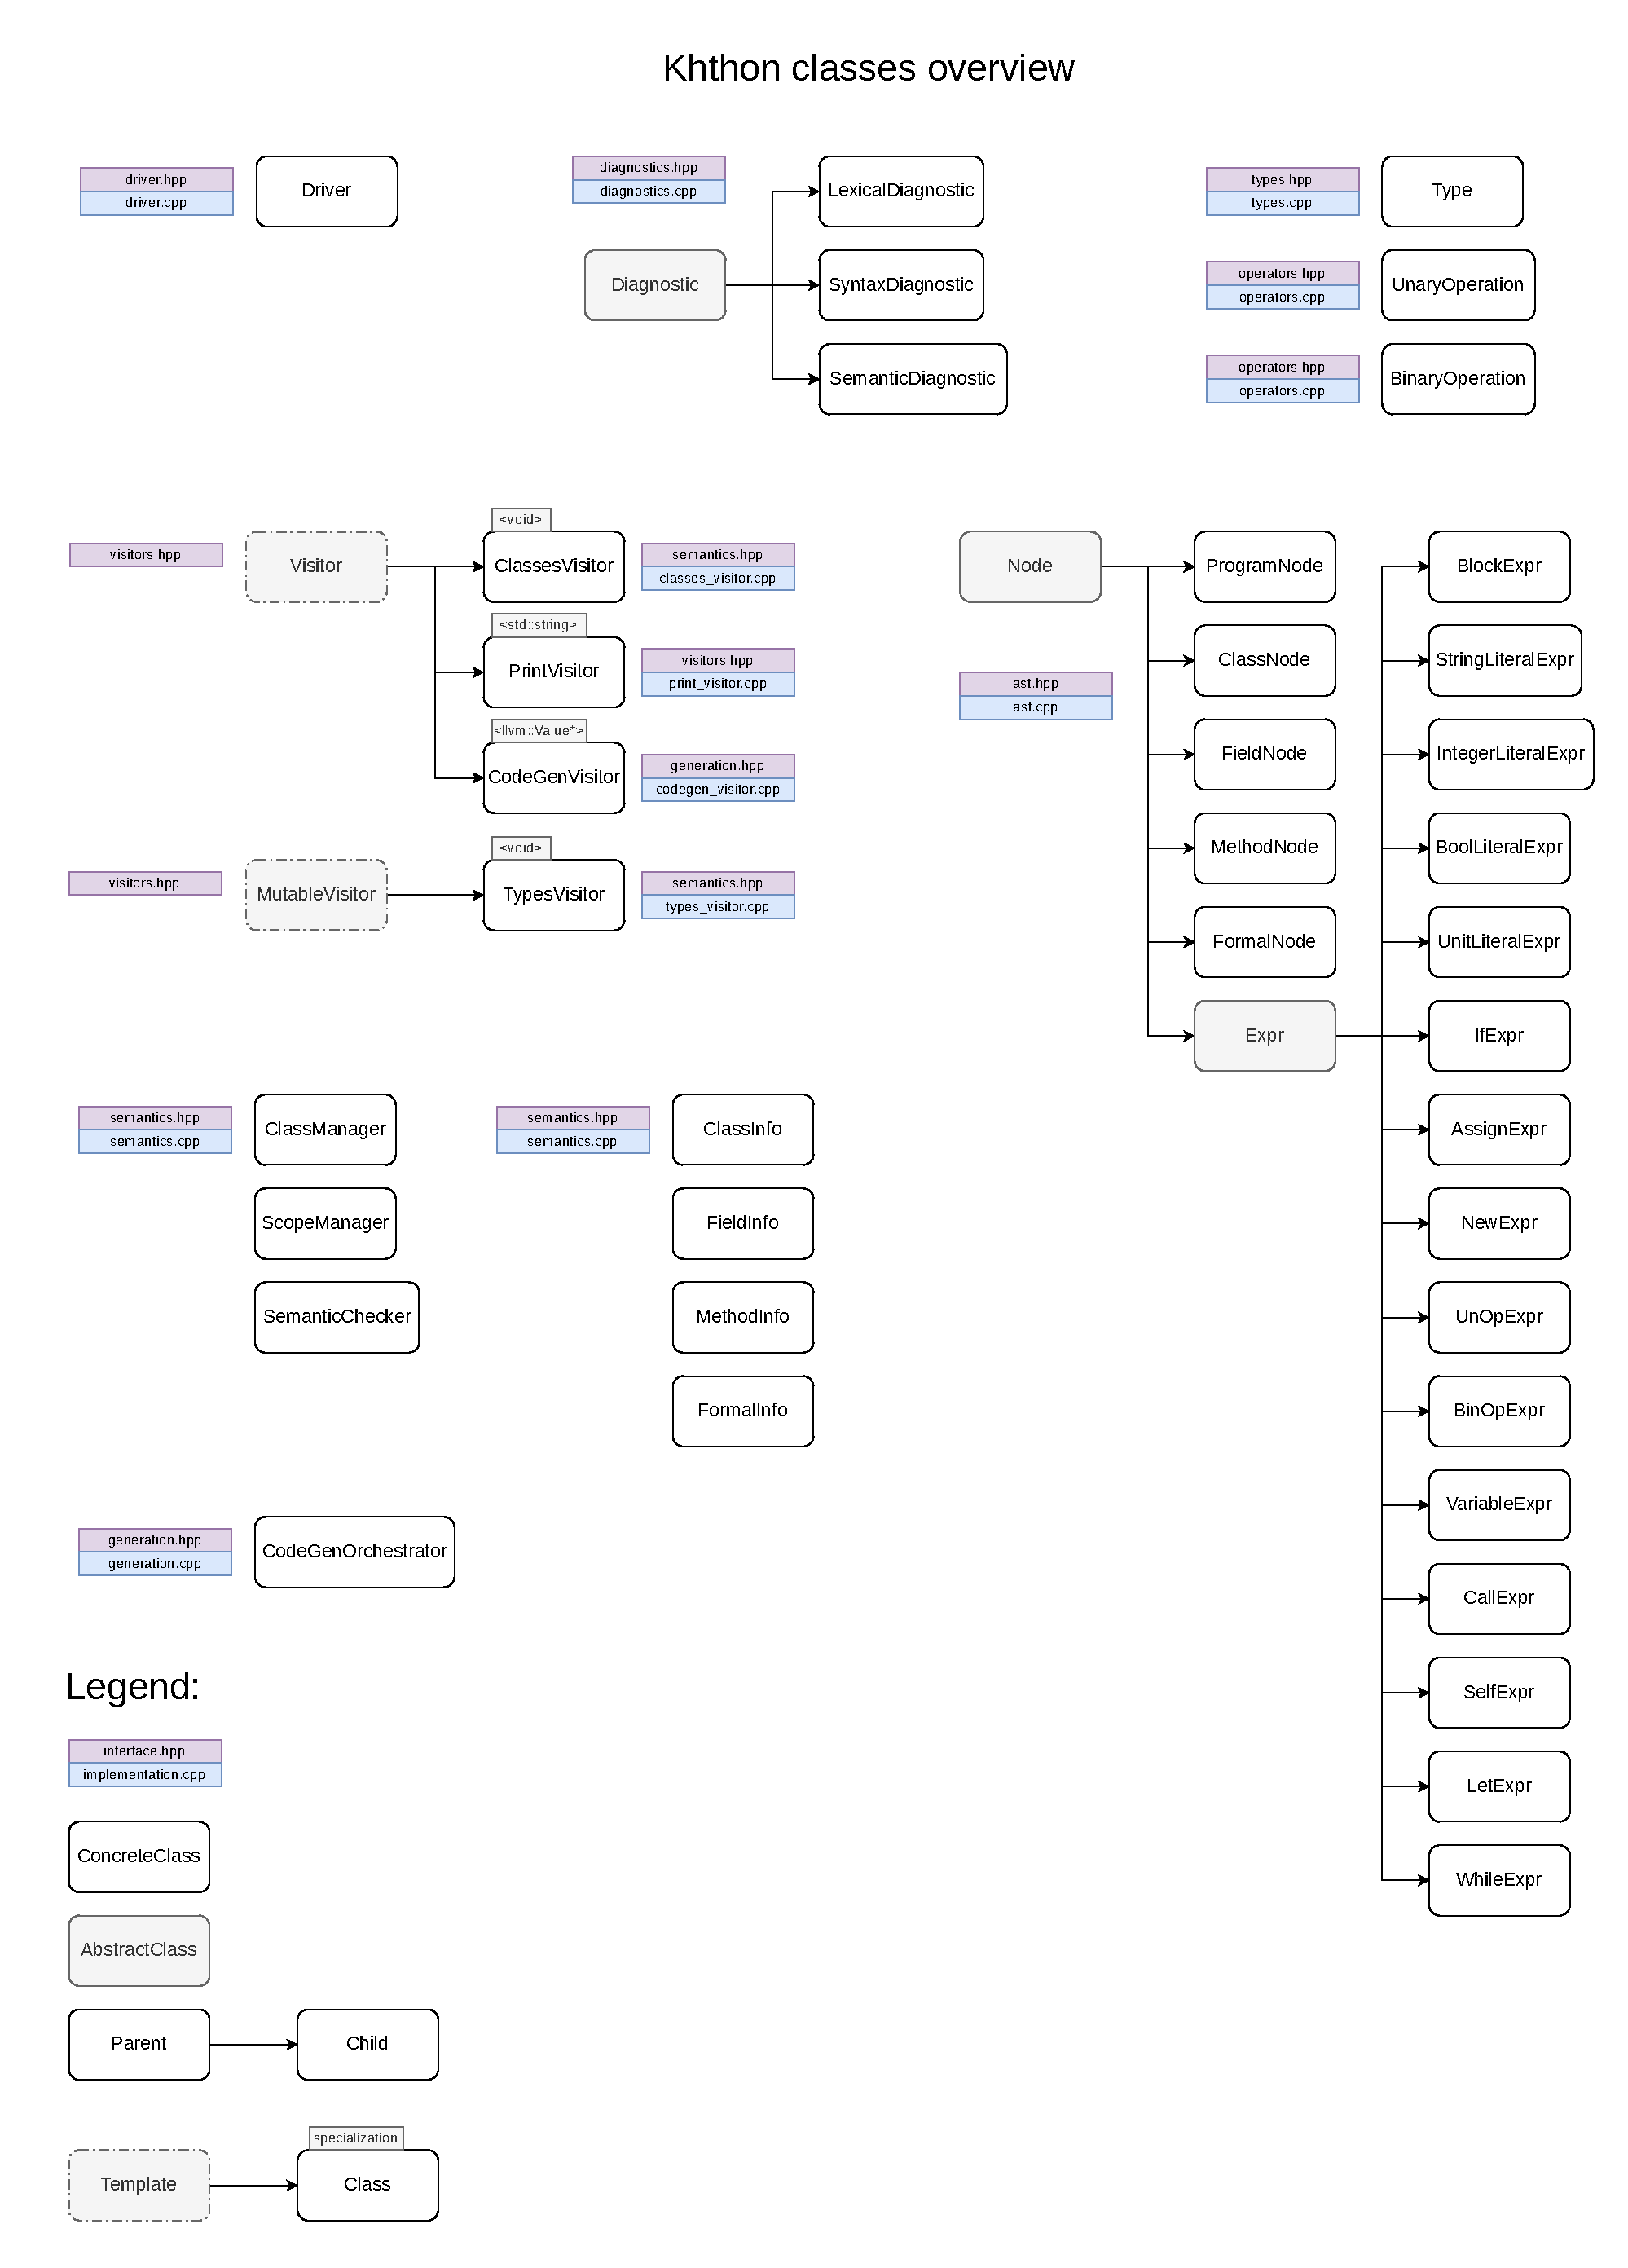
\includepdf{images/schematics/overview.pdf}

\end{document}
